\documentclass[aspectratio=169,11pt]{beamer}
\usepackage[utf8]{inputenc}
\usepackage[T1]{fontenc}
\usepackage[spanish]{babel}
\usepackage{amsmath,amssymb}
\usepackage{tikz}
\usetikzlibrary{arrows.meta,angles,calc,positioning}
\usetheme{Madrid}
\usecolortheme{default}
\setbeamertemplate{navigation symbols}{}
\setbeamertemplate{blocks}[rounded][shadow=false]
\newcommand{\ang}[1]{\angle #1^\circ}

\title[Algoritmos de QFT]{Paso 16: Algoritmos de QFT}
\subtitle{Cómo funciona por dentro lo que hicimos a mano en los pasos 7 a 9}
\author{Curso de control robusto (QFT)}
\date{}
\begin{document}
\begin{frame}\titlepage\end{frame}

\begin{frame}{Dónde encaja este paso}
  \tiny
  \begin{enumerate}\setlength{\itemsep}{-2pt}
    \item[1.] Números complejos \hfill \textcolor{gray}{(hecho)}
    \item[2.] Funciones de transferencia: $s$, polos y ceros \hfill \textcolor{gray}{(hecho)}
    \item[3.] Respuesta en frecuencia: $s=j\omega$, magnitud y fase \hfill \textcolor{gray}{(hecho)}
    \item[4.] Decibelios y escala logarítmica (Bode) \hfill \textcolor{gray}{(hecho)}
    \item[5.] Realimentación: $L$, $T=\frac{L}{1+L}$, $S=\frac{1}{1+L}$ \hfill \textcolor{gray}{(hecho)}
    \item[6.] Nichols chart \hfill \textcolor{gray}{(hecho)}
    \item[7.] Incertidumbre y templates \hfill \textcolor{gray}{(hecho)}
    \item[8.] Especificaciones $\rightarrow$ bounds \hfill \textcolor{gray}{(hecho)}
    \item[9.] Loop shaping, prefiltro y verificación \hfill \textcolor{gray}{(hecho)}
    \item[10.] QFT en control digital \hfill \textcolor{gray}{(hecho)}
    \item[11.] Dos caminos digitales: $z$ y $w$ \hfill \textcolor{gray}{(hecho)}
    \item[12.] Estabilidad, límites, más especificaciones y caso real \hfill \textcolor{gray}{(hecho)}
    \item[13.] Muestreo por eventos con periodo base $T$ \hfill \textcolor{gray}{(hecho)}
    \item[14.] Sistemas de dos estados: lazo interno y externo \hfill \textcolor{gray}{(hecho)}
    \item[15.] QFT y sistemas no lineales \hfill \textcolor{gray}{(hecho)}
    \item[\textbf{16.}] \textbf{Algoritmos de QFT: cómo funcionan por dentro} \hfill $\leftarrow$ estamos aquí
    \item[17.] QFT en Python: una biblioteca paso a paso
    \item[18.] QFT en MATLAB: el mismo código, otra sintaxis
    \item[19.] Historia, panorama y bibliografía
  \end{enumerate}
  \vspace{2pt}
  \begin{block}{Objetivo de hoy}
    \footnotesize
    Hasta ahora usamos los resultados (templates, bounds, $L_0$). Aquí se abre la caja: \textbf{qué algoritmo} hay detrás de cada uno, cuánto cuesta, qué errores comete y cuándo da resultados falsos. Los pasos 17 y 18 lo programan en Python y MATLAB.
  \end{block}
\end{frame}

\begin{frame}{La tubería de QFT en seis algoritmos}
  \small
  \centering
  \begin{tikzpicture}[>=Stealth,node distance=0.35cm,box/.style={draw,rounded corners,minimum height=1.0cm,minimum width=2.05cm,font=\scriptsize,align=center,fill=blue!6}]
    \node[box] (a) {1. Familia\\y templates};
    \node[box,right=of a] (b) {2. Mapas\\de bounds};
    \node[box,right=of b] (c) {3. Loop\\shaping};
    \node[box,right=of c] (d) {4. Prefiltro};
    \node[box,right=of d,fill=orange!15] (e) {5. Verificación};
    \draw[->] (a)--(b); \draw[->] (b)--(c); \draw[->] (c)--(d); \draw[->] (d)--(e);
    \draw[->,dashed] (e.south) |- ++(0,-0.6) -| node[near start,below,font=\scriptsize]{si falla: añadir $\omega$ y repetir} (b.south);
  \end{tikzpicture}
  \vspace{4pt}
  \begin{center}\footnotesize
  \begin{tabular}{l|l|l}
    Algoritmo & Entra & Sale\\\hline
    Templates & $P(j\omega,\theta)$, rejilla de $\theta$ & $N$ puntos complejos por $\omega$\\
    Mapas de bounds & templates, especificaciones & mapa de fase$\times$módulo permitido\\
    Loop shaping & mapas, forma de $G$ & $(k,z,p)$ o una curva $L_0$\\
    Prefiltro & $G$, banda $[T_L,T_U]$ & polo $f$ de $F$\\
    Verificación & $G$, $F$, familia & frecuencias que fallan, polos
  \end{tabular}
  \end{center}
  \footnotesize El bucle de la derecha es lo que más se olvida: el diseño \textbf{solo} es válido en las frecuencias que se calcularon.
\end{frame}

\begin{frame}{Algoritmo 1: templates y el borde de la caja}
  \footnotesize
  \begin{columns}[T]
  \begin{column}{0.52\textwidth}
    Para cada $\omega$ de la lista:
    \begin{enumerate}
      \item Evaluar $P(j\omega,\theta_i)$ para toda la rejilla ($17\times13=221$ plantas).
      \item Dividir por el nominal: $r_i=P_i/P_0$.
      \item Quedarse con las plantas que \textbf{tienen algún parámetro en un extremo} de su rango.
    \end{enumerate}
    \vspace{2pt}
    En el ejemplo son $56$ de $221$. Para estas especificaciones, comprobar solo esas plantas da \textbf{exactamente} el mismo resultado que comprobarlas todas, y cuesta $4\times$ menos.
  \end{column}
  \begin{column}{0.46\textwidth}
    \begin{alertblock}{Una trampa}
      Tomar la \textbf{envolvente convexa} del template (15 puntos) parece lo natural, pero \textbf{no es seguro}: el mapa resultante da por válidas celdas que no lo son (siguiente diapositiva).
    \end{alertblock}
  \end{column}
  \end{columns}
\end{frame}

\begin{frame}{Template y mapa: la trampa de la envolvente convexa}
  \footnotesize
  \centering
  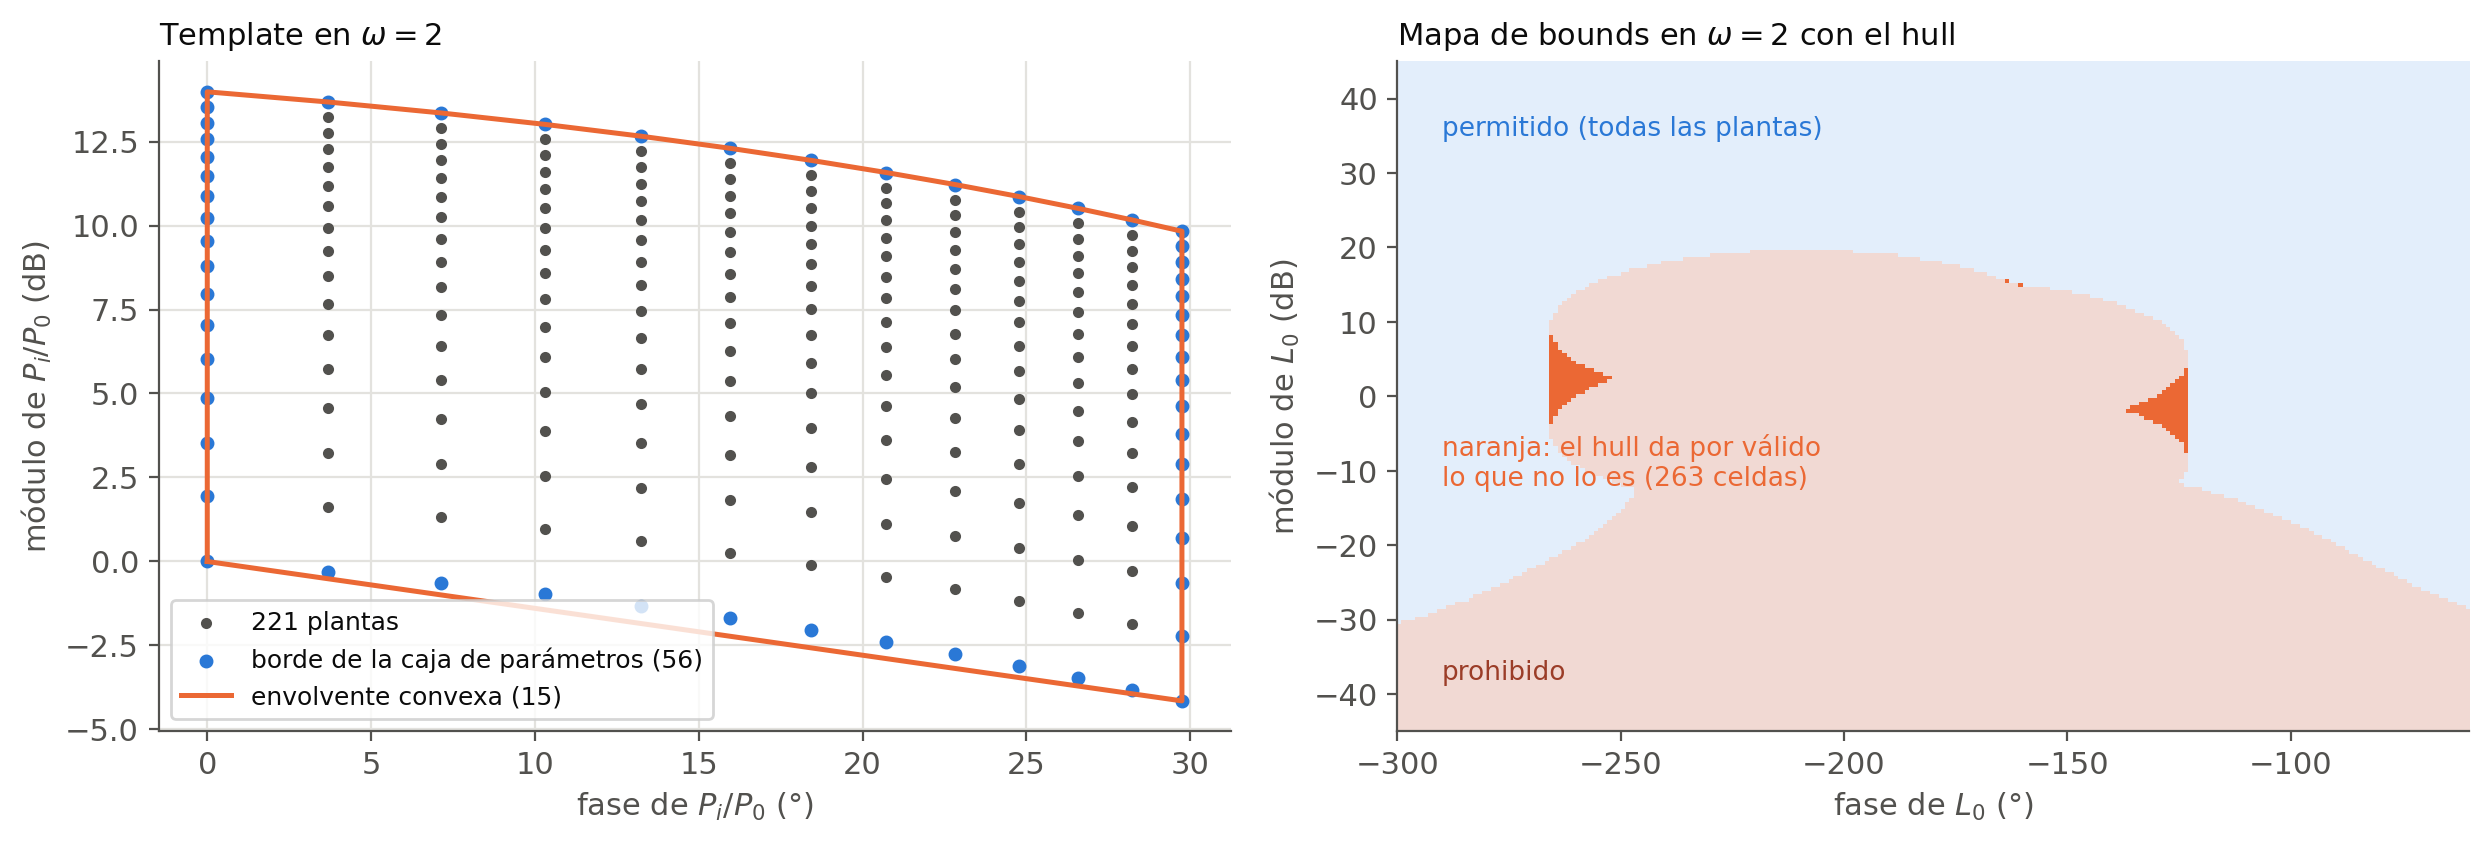
\includegraphics[width=\textwidth]{fig/template_hull.png}\\[2pt]
  Izquierda: las 221 plantas, el borde de la caja (azul) y la envolvente convexa (naranja). Derecha: el mapa en $\omega=2$; lo naranja son celdas que el hull da por válidas y \textbf{no lo son}.
\end{frame}

\begin{frame}{Qué cuesta cada elección}
  \small
  \begin{center}
  \begin{tabular}{l|c|c|c}
    Plantas usadas & Nº & Celdas erróneas ($\omega=2$) & Tiempo por mapa\\\hline
    Todas & 221 & 0 & 1004 ms\\
    Borde de la caja de parámetros & 56 & \textbf{0} & 231 ms\\
    Envolvente convexa del template & 15 & \textbf{263} & 58 ms
  \end{tabular}
  \end{center}
  \footnotesize
  Celdas erróneas = celdas que el mapa con esas plantas da por permitidas y el mapa completo prohíbe. En otras frecuencias: $\omega=0.1$: 21; $\omega=1$: 3; $\omega=5$: 261; $\omega=20$: 260 (sobre $86\,760$ celdas).
  \begin{itemize}
    \item La envolvente convexa vale para especificaciones \textbf{monótonas} en el template. El seguimiento mide una \textbf{dispersión} (máximo menos mínimo de $|T_i|$), que no lo es: los extremos pueden estar dentro del contorno.
    \item Regla práctica: si no se ha comprobado, usar \textbf{todas} las plantas o el borde de la caja.
    \item Medidas sobre este ordenador (un hilo, NumPy): sirven para comparar, no como cifras absolutas.
  \end{itemize}
\end{frame}

\begin{frame}{Algoritmo 2: el mapa de bounds por rejilla}
  \footnotesize
  Para una frecuencia $\omega$ y un nominal $P_0$, se calcula un \textbf{mapa booleano} sobre $(\varphi,\,m)$ = (fase, módulo en dB) de $L_0$:
  \begin{block}{Pseudocódigo}
    \begin{tabbing}
    \hspace{0.5cm}\=\hspace{0.5cm}\=\kill
    para cada fase $\varphi\in\{-360,\dots,-1\}$ (paso $1^\circ$):\\
    \> para cada módulo $m\in\{-60,\dots,60\}$ (paso 0.5 dB):\\
    \>\> $L_0\leftarrow10^{m/20}e^{j\varphi}$;\quad $L_i\leftarrow L_0\,r_i$ para todas las plantas del borde\\
    \>\> mapa$[\varphi,m]\leftarrow$ \textbf{todas} las especificaciones se cumplen para \textbf{todas} las $L_i$
    \end{tabbing}
  \end{block}
  \begin{itemize}
    \item Coste: $360\times241\times56\approx4.9$ millones de evaluaciones por especificación y por $\omega$. Se vectoriza (matrices 3D) y tarda $\sim0.2$ s.
    \item Cada especificación da su mapa; la \textbf{intersección} (AND lógico) es el mapa final. Es la figura siguiente.
    \item Lo que en los pasos 7 y 8 se dibujaba como ``contorno'' es la \textbf{frontera} de este mapa.
  \end{itemize}
\end{frame}

\begin{frame}{Los mapas en $\omega=1$ y la curva $L_0$}
  \footnotesize
  \begin{columns}[T]
  \begin{column}{0.62\textwidth}
    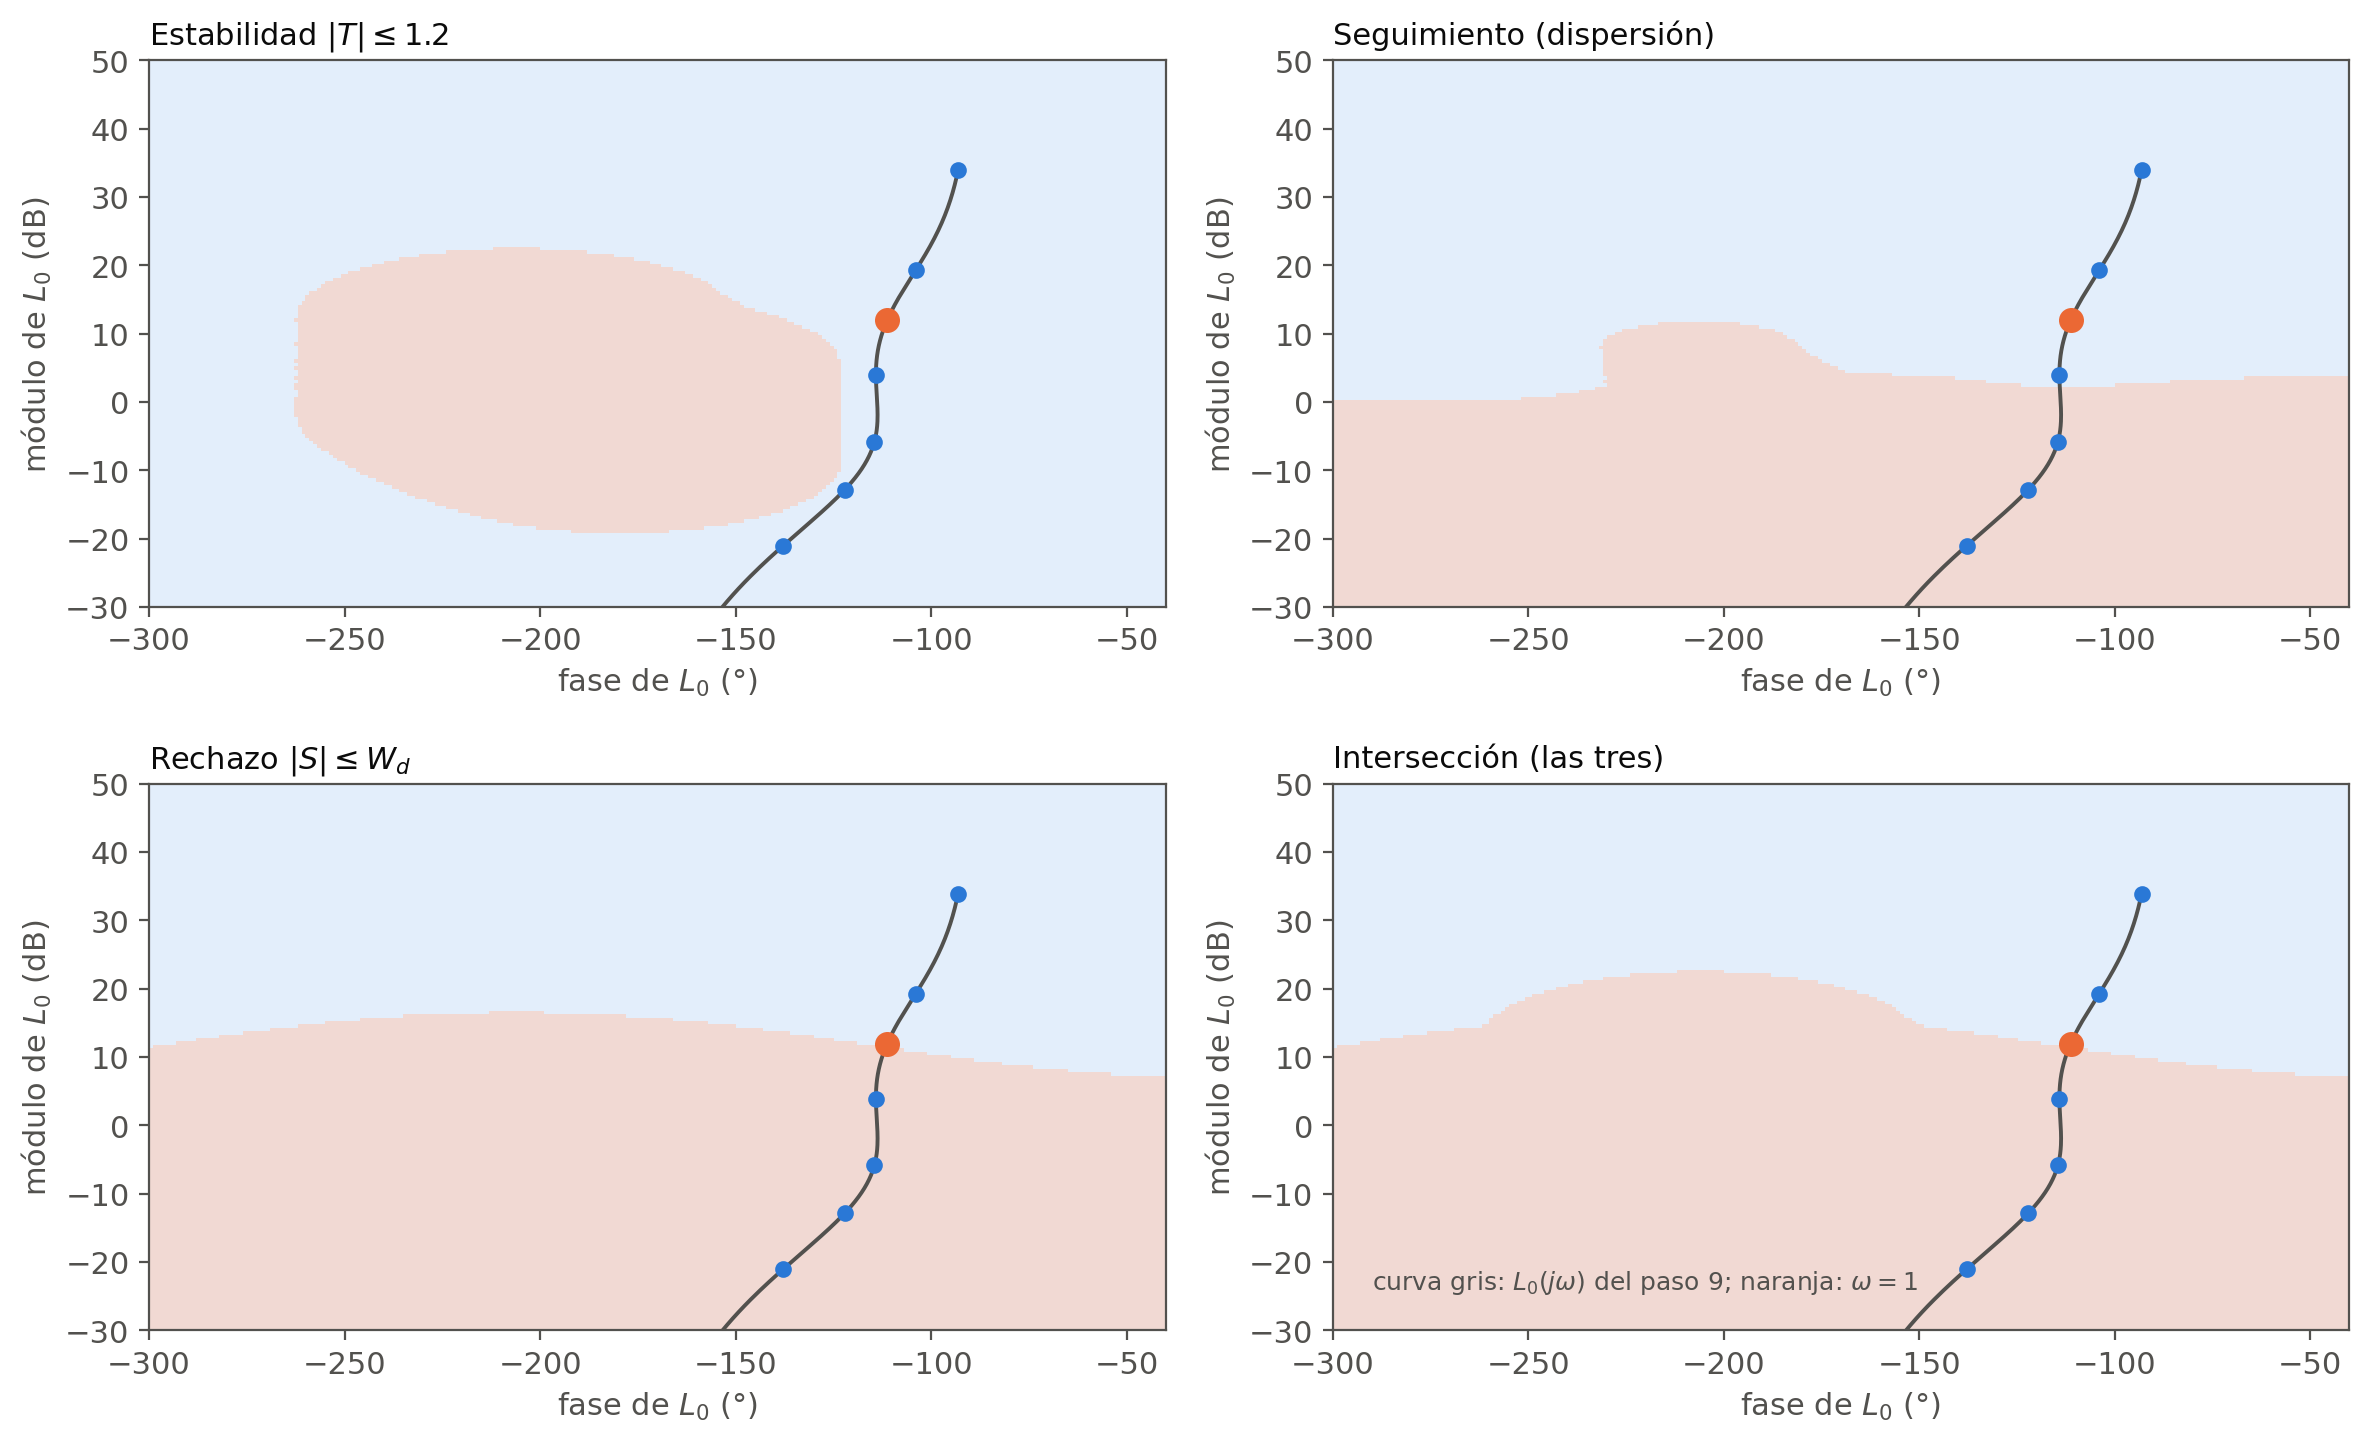
\includegraphics[width=\textwidth]{fig/mapas_specs.png}
  \end{column}
  \begin{column}{0.36\textwidth}
    Azul: permitido. Rosa: prohibido. Puntos azules: $L_0(j\omega)$ del paso 9 en las 8 frecuencias de diseño; el naranja es $\omega=1$.
    \begin{itemize}
      \item En $\omega=1$ el punto queda \textbf{a $0.93$ dB} de la frontera: lo limita el rechazo de perturbación.
      \item La estabilidad ($|T|\le1.2$) es una región \textbf{cerrada} alrededor de $-180^\circ$; las otras dos son un suelo de ganancia.
    \end{itemize}
  \end{column}
  \end{columns}
\end{frame}

\begin{frame}{Una fórmula cerrada para el bound de estabilidad}
  \small
  Para una planta con $u=r_i\,e^{j\varphi}$ y $L=x\,u$ con $x=|L_0|>0$, la condición $|T|>W_s$ ($W_s>1$) es
  \[ A\,x^2+2W_s^2\,\mathrm{Re}(u)\,x+W_s^2\ge0,\qquad A=(W_s^2-1)|u|^2 \]
  \begin{itemize}
    \item Se incumple $|T|\le W_s$ cuando $x$ está \textbf{entre las dos raíces} (si el discriminante es positivo y $\mathrm{Re}(u)<0$):
    \[ x_{\pm}=\frac{-W_s^2\,\mathrm{Re}(u)\pm\sqrt{W_s^2\big(W_s^2\mathrm{Re}(u)^2-(W_s^2-1)|u|^2\big)}}{A}. \]
    \item El intervalo prohibido de $|L_0|$ en esa fase es la \textbf{unión} de estos intervalos sobre las plantas.
  \end{itemize}
  \begin{block}{Comprobación}
    Frente al mapa por rejilla (86\,760 celdas), esta fórmula da \textbf{0 celdas distintas} en $\omega=1$ y en $\omega=2$. Sirve como \textbf{test} del código de rejilla.
  \end{block}
  \footnotesize El seguimiento parece no tener fórmula cerrada (es un máximo menos un mínimo), pero \textbf{sí} la tiene si se compara por \textbf{pares} de plantas: siguiente diapositiva.
\end{frame}

\begin{frame}{Bounds exactos: una desigualdad cuadrática por especificación}
  \small
  Con $L=x\,u_i$, $x=|L_0|$ y $u_i=r_i e^{j\varphi}$ ($r_i=P_i/P_0$), \textbf{cada} especificación se reduce a $a\,x^2+b\,x+c\ge0$:
  \begin{center}\footnotesize
  \begin{tabular}{lccc}
    \hline
    Especificación & $a$ & $b$ & $c$\\
    \hline
    $|T|\le W_s$ & $(W_s^2-1)|u|^2$ & $2W_s^2\,\mathrm{Re}\,u$ & $W_s^2$\\
    $|S|\le W_d$ & $W_d^2|u|^2$ & $2W_d^2\,\mathrm{Re}\,u$ & $W_d^2-1$\\
    $|T_d|\le R\,|T_e|$ & $(R^2-1)|u_d|^2|u_e|^2$ & $2\big(R^2|u_e|^2\mathrm{Re}\,u_d-|u_d|^2\mathrm{Re}\,u_e\big)$ & $R^2|u_e|^2-|u_d|^2$\\
    \hline
  \end{tabular}
  \end{center}
  \begin{itemize}
    \item Para cada fase y cada planta (o par $(d,e)$) se resuelve la cuadrática: el conjunto prohibido de $x$ es un \textbf{intervalo} (o el complemento de uno).
    \item El bound en esa fase es la \textbf{unión ordenada} de intervalos: se ordenan por extremo inferior y se funden los que se solapan.
    \item La dispersión de seguimiento $\max_i|T_i|/\min_i|T_i|\le R$ equivale a que \textbf{todos} los pares cumplan $|T_d|\le R|T_e|$: son $N(N-1)$ cuadráticas.
  \end{itemize}
  \footnotesize Es la idea de los bounds \emph{exactos} de Chait y Yaniv (1993) y de su extensión a varias especificaciones (Rodrigues, Chait y Yaniv, 1997): ni rejilla de módulo ni error de discretización.
\end{frame}

\begin{frame}{Exacto frente a rejilla: márgenes y coste}
  \small
  Mismo $G(s)=5\frac{1+s/2}{1+s/20}$, mismas 56 plantas del borde, las 8 frecuencias del ejemplo:
  \begin{center}\footnotesize
  \begin{tabular}{lcccccccc}
    \hline
    $\omega$ & 0.1 & 0.5 & 1 & 2 & 5 & 10 & 20 & 50\\
    \hline
    Rejilla 0.5 dB & 6.45 & 0.79 & 0.93 & 17.94 & $\ge$60 & $\ge$60 & 5.54 & 16.12\\
    Exacto & 6.29 & 0.70 & 0.63 & 17.67 & $\ge$60 & $\ge$60 & 5.22 & 16.08\\
    \hline
  \end{tabular}
  \end{center}
  \begin{itemize}
    \item Margen en dB; \textbf{la rejilla sobrestima} siempre ($0.1$ a $0.3$ dB): es la celda, no un fallo del código.
    \item \textbf{Coincidencia celda a celda}: si se evalúa el intervalo exacto en los puntos de la rejilla, hay \textbf{0 celdas distintas} en seis frecuencias. El exacto es más preciso, no distinto.
    \item Coste: unos $1$ ms por margen frente a $0.2$--$0.3$ s por mapa. Pero el mapa sirve para \textbf{dibujar} el bound; el exacto, para \textbf{decidir} si $L_0$ cumple.
  \end{itemize}
  \begin{alertblock}{Consecuencia para el diseño}
    En $\omega=1$ el margen real es $0.63$ dB y no $0.93$ dB. Un diseño que fuera justo con la rejilla podría quedar \textbf{dentro} del bound exacto: en el límite, conviene usar el exacto para la verificación final.
  \end{alertblock}
\end{frame}

\begin{frame}{Margen y comprobación de $L_0$}
  \small
  Dado el mapa de una frecuencia y un punto $(\varphi_0,m_0)$ de $L_0$:
  \begin{enumerate}
    \item Elegir la columna de fase más cercana (\textbf{módulo $360^\circ$}: $-359^\circ$ y $+1^\circ$ son la misma fase).
    \item Si la celda es permitida: margen $=$ distancia vertical (dB) a la celda prohibida más cercana. Si no: margen negativo $=$ distancia a la permitida más cercana.
    \item Si la columna no tiene celdas de otro tipo: se trunca a $\pm60$ dB.
  \end{enumerate}
  \begin{itemize}
    \item En el ejemplo, con $G(s)=5\frac{1+s/2}{1+s/20}$ los márgenes en las 8 frecuencias son
    \[ 6.45,\;0.79,\;0.93,\;17.94,\;\ge60,\;\ge60,\;5.54,\;16.12\ \text{dB}. \]
    \item El mínimo de estos márgenes ($0.79$ dB en $\omega=0.5$) es el \textbf{margen de diseño}: lo que se maximiza o se exige positivo.
    \item Margen vertical, no distancia en el plano: es la que importa, porque cambiar la ganancia $k$ mueve $L_0$ \textbf{en vertical}.
  \end{itemize}
\end{frame}

\begin{frame}{Algoritmo 3: loop shaping automático}
  \footnotesize
  Se parametriza $G(s)=k\,\frac{1+s/z}{1+s/p}$ y se busca por \textbf{evolución diferencial} (algoritmo global que no necesita derivadas):
  \[ \min_{k,z,p}\ \underbrace{\frac{kp}{z}}_{G(\infty)}+10^3\sum_\omega\max\big(0,-\text{margen}(\omega)\big),\qquad 0.5\le k\le30,\ 0.2\le z\le20,\ 2\le p\le200. \]
  \begin{itemize}
    \item Objetivo: la menor \textbf{ganancia de alta frecuencia} (menos ruido y esfuerzo, pasos 12 y 14).
    \item La penalización suma los dB de violación: guía al algoritmo hacia lo permitido.
    \item Es un \textbf{problema no convexo}: depende de la semilla; conviene repetir con varias.
  \end{itemize}
  \begin{alertblock}{Pero con solo 8 frecuencias engaña}
    Primera iteración: $k=5.00$, $z=2.22$, $p=13.1$, $G(\infty)=29.6$, y \textbf{33 de 400} frecuencias de la verificación densa fallan. El diseño cumple en las $\omega$ elegidas y \textbf{no} entre ellas.
  \end{alertblock}
\end{frame}

\begin{frame}{El bucle de refinado}
  \footnotesize
  \begin{block}{Algoritmo}
    \begin{tabbing}
    \hspace{0.5cm}\=\kill
    $\Omega\leftarrow$ 8 frecuencias iniciales\\
    repetir (máx. 8 veces):\\
    \> calcular los mapas en $\Omega$;\quad $(k,z,p)\leftarrow$ evolución diferencial\\
    \> fallos $\leftarrow$ verificación densa de las 221 plantas en 400 frecuencias\\
    \> si no hay fallos: terminar\\
    \> añadir a $\Omega$ 3 frecuencias de los fallos (repartidas)
    \end{tabbing}
  \end{block}
  \begin{center}
  \begin{tabular}{c|c|c|c|c}
    Iteración & $k,\,z,\,p$ & $G(\infty)$ & Fallos & $|\Omega|$\\\hline
    1 & $5.00,\ 2.22,\ 13.1$ & 29.6 & 33 & 8\\
    2 & $5.13,\ 2.65,\ 16.6$ & 32.1 & 16 & 11\\
    3 & $5.08,\ 2.47,\ 16.1$ & 33.1 & 6 & 14\\
    4 & $5.10,\ 2.54,\ 16.6$ & 33.3 & 1 & 17\\
    8 & $5.10,\ 2.52,\ 16.4$ & 33.2 & \textbf{0} & 21
  \end{tabular}
  \end{center}
  \footnotesize A mano (paso 9) $G(\infty)=50$; el algoritmo consigue $\approx33$ con 21 frecuencias.
\end{frame}

\begin{frame}{Algoritmos 4 y 5: prefiltro y verificación}
  \small
  \begin{columns}[T]
  \begin{column}{0.49\textwidth}
    \begin{block}{Prefiltro $F=\frac{1}{1+s/f}$}
      \footnotesize
      Para cada $f$ de una rejilla: margen mínimo (dB) entre $|T_iF|$ y la banda $[T_L,T_U]$ en todas las plantas y frecuencias. Elegir la $f$ de mayor margen.
      \begin{itemize}
        \item $G$ del paso 9: $f=1.1$, margen $0.028$ dB.
        \item $G$ automático: $f=1.0$, margen $0.032$ dB.
      \end{itemize}
    \end{block}
  \end{column}
  \begin{column}{0.49\textwidth}
    \begin{block}{Verificación}
      \footnotesize
      \begin{itemize}
        \item Las tres especificaciones en las 221 plantas y 400 frecuencias.
        \item \textbf{Estabilidad}: polos de $1+L=0$ de cada planta ($s(s+a)(s+p)+Kk\frac{p}{z}(s+z)=0$).
        \item Peor polo de la familia: $\mathrm{Re}=-1.19$ (paso 9) y $-1.51$ (automático).
      \end{itemize}
    \end{block}
  \end{column}
  \end{columns}
  \vspace{3pt}
  \footnotesize La verificación densa \textbf{no es opcional}: es lo que detecta los fallos entre frecuencias de diseño y la que cierra el bucle de refinado.
\end{frame}

\begin{frame}{Resolución de las rejillas y coste}
  \footnotesize
  \centering
  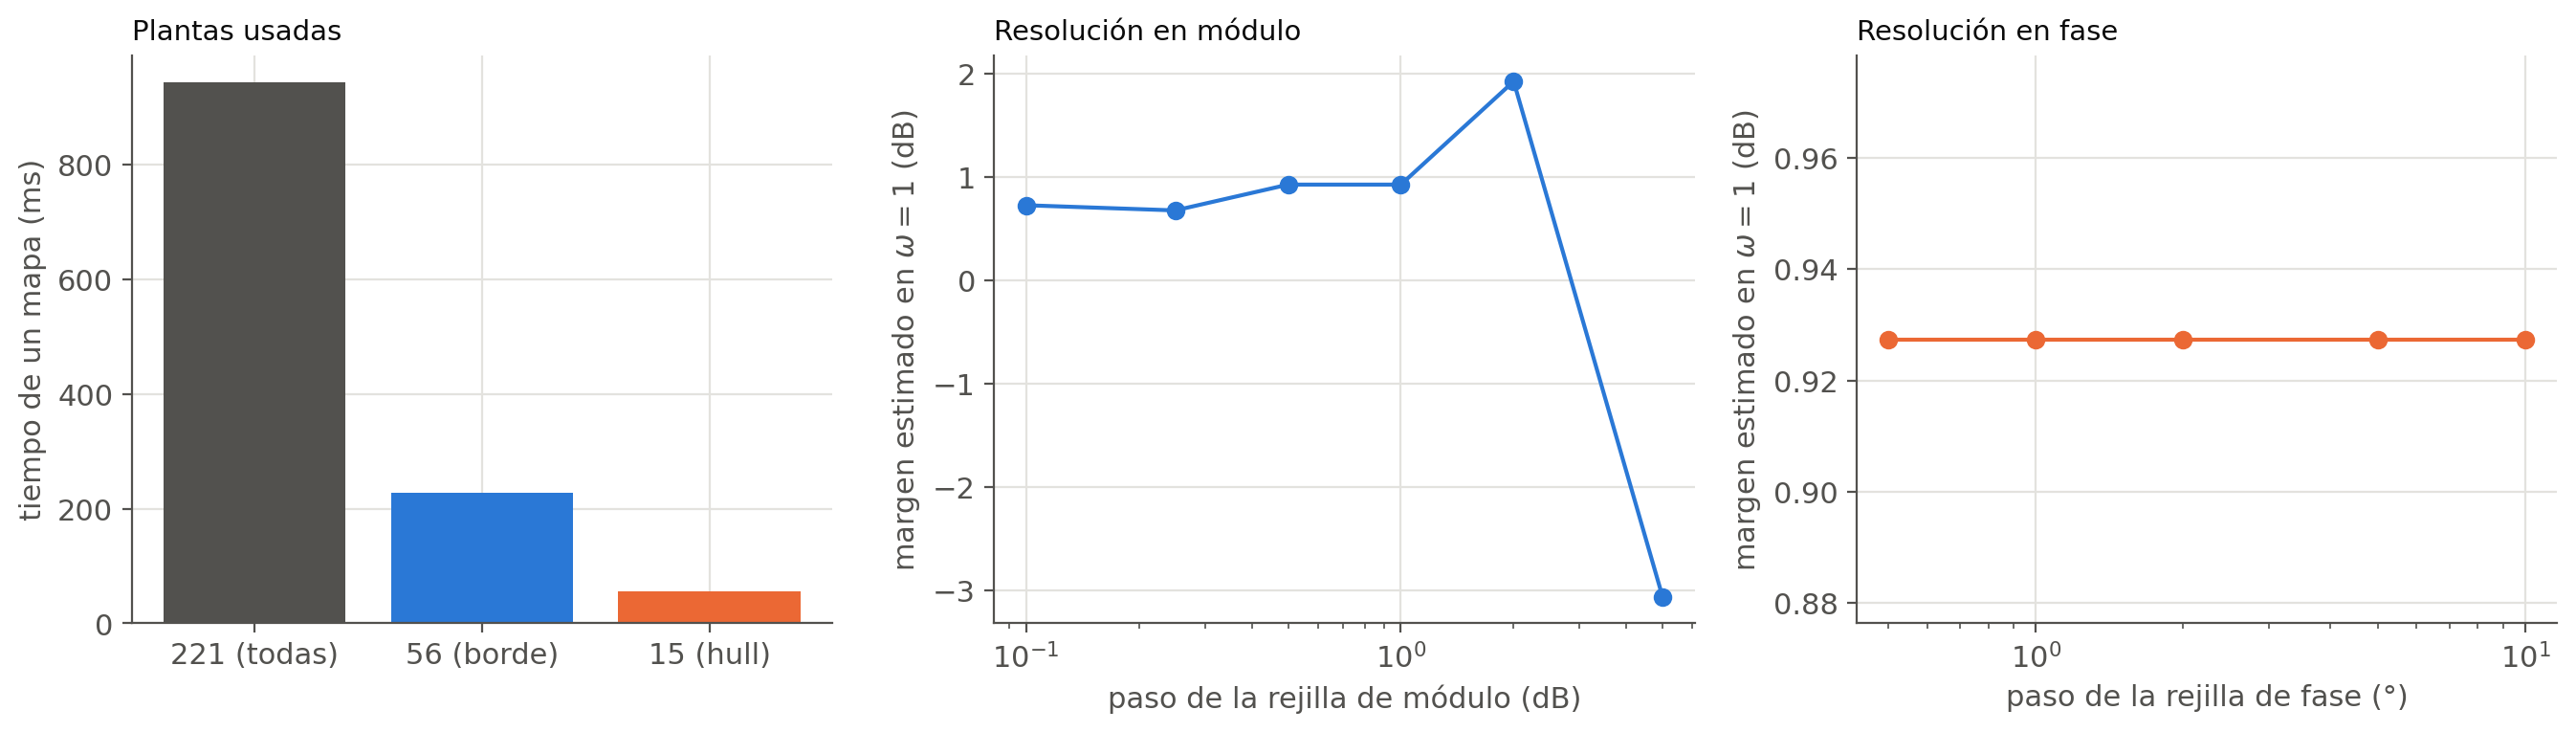
\includegraphics[width=\textwidth]{fig/coste_resolucion.png}\\[2pt]
  \begin{itemize}
    \item \textbf{Módulo}: el margen en $\omega=1$ es $0.73$ dB con paso $0.1$ dB, $0.93$ con $0.5$, $1.93$ con $2$ y $-3.07$ con $5$ (dice que \textbf{no cumple}). Paso 0.5 dB sobreestima en $\sim0.2$ dB.
    \item \textbf{Fase}: casi no importa aquí ($0.93$ dB para pasos de $0.5^\circ$ a $10^\circ$); la frontera cambia poco con la fase en ese punto.
    \item El tiempo crece con el producto de las dos rejillas: paso $0.1$ dB cuesta $1.3$ s por mapa; $2$ dB, $42$ ms.
  \end{itemize}
\end{frame}

\begin{frame}{En discreto: qué cambia en el algoritmo}
  \small
  \begin{center}
  \begin{tabular}{l|l|l}
    & Continuo & Discreto (plano $w$)\\\hline
    Evaluar $P$ & $P(j\omega)$ & $P(w)$ con $w=j\nu$, $\nu=\frac{2}{T_s}\tan\frac{\omega T_s}{2}$\\[2pt]
    Rango de frecuencias & hasta donde se quiera & hasta Nyquist, $\omega<\pi/T_s$\\[2pt]
    Especificaciones & en $\omega$ & en $\omega$ real (pre-warping), no en $\nu$\\[2pt]
    Mapas y bounds & el mismo algoritmo & \textbf{el mismo algoritmo}\\[2pt]
    Verificación & $L(j\omega)$ & $L(e^{j\omega T_s})$, y polos con $|z|<1$
  \end{tabular}
  \end{center}
  \begin{itemize}
    \item El código de mapas, margen y refinado \textbf{no cambia}: solo cambia la función $P(\cdot)$ que se le pasa y la lista de frecuencias.
    \item Esa es la ventaja del plano $w$ (paso 11): se reutiliza todo el software continuo.
  \end{itemize}
\end{frame}

\begin{frame}{Errores típicos al programar QFT}
  \footnotesize
  \begin{enumerate}
    \item \textbf{Fase sin envolver}: usar $+170^\circ$ en lugar de $-190^\circ$. Siempre módulo $360^\circ$.
    \item \textbf{Dividir por el nominal mal}: el template relativo es $P_i/P_0$ con el \textbf{mismo} $\omega$.
    \item \textbf{Envolvente convexa sin comprobar} (paso 16, diapositivas 4 y 5).
    \item \textbf{Pocas frecuencias}: el diseño pasa en ellas y falla entre medias.
    \item \textbf{Rejilla de módulo gruesa}: sobreestima o subestima márgenes de décimas de dB.
    \item \textbf{Cambiar el número de polos inestables} de la familia: Nyquist dice otra cosa (paso 12). Los mapas no lo detectan.
    \item \textbf{Mezclar unidades}: $|T|\le1.2$ es $1.58$ dB; $W_d$ es módulo, no dB.
    \item \textbf{Especificaciones en $\nu$}, no en $\omega$, en discreto.
  \end{enumerate}
  \begin{alertblock}{Una regla}
    Todo algoritmo de esta lista tiene un \textbf{test}: la fórmula cerrada del bound de estabilidad, los bounds exactos frente a la rejilla, la verificación densa con las 221 plantas, y los polos del lazo cerrado.
  \end{alertblock}
\end{frame}

\begin{frame}{Resumen}
  \small
  \begin{itemize}
    \item QFT en código son \textbf{cinco algoritmos}: templates, mapas de bounds, loop shaping, prefiltro y verificación, con un bucle de refinado.
    \item El mapa de bounds es un \textbf{cálculo por rejilla} de fase$\times$módulo; el borde de la caja de parámetros basta, la envolvente convexa \textbf{no}.
    \item Loop shaping automático por evolución diferencial: $G(\infty)\approx33$ frente a $50$ a mano, pero \textbf{solo} tras refinar con verificación densa.
    \item Rejilla de módulo de $0.5$ dB: error de $\sim0.2$ dB en el margen; los \textbf{bounds exactos} (una cuadrática por especificación) lo eliminan y coinciden celda a celda con la rejilla.
    \item En discreto el algoritmo es el mismo: cambia $P(\cdot)$ y la lista de frecuencias.
  \end{itemize}
  \begin{block}{Ejercicio}
    (1) ¿Cuántas evaluaciones de $T$ hace un mapa con paso de módulo $1$ dB y de fase $2^\circ$ con las 56 plantas del borde y 3 especificaciones? (2) ¿Por qué $-359^\circ$ y $+1^\circ$ comparten columna? (3) ¿Por qué la envolvente convexa no sirve para una especificación de dispersión?
  \end{block}
\end{frame}

\appendix
\begin{frame}{Solución del ejercicio}
  \footnotesize
  \textbf{1.} Fases: $360/2=180$. Módulos: $-60$ a $60$ en pasos de $1$: $121$. Celdas: $180\cdot121=21\,780$. Evaluaciones: $21\,780\cdot56\cdot3=3\,659\,040$ (unos 3.7 millones).\\[3pt]
  \textbf{2.} La fase de $L_0$ solo importa módulo $360^\circ$: $e^{j(-359^\circ)}=e^{j(1^\circ)}$. Con la rejilla en $[-360,0)$ se lleva todo ese rango con \texttt{mod}.\\[3pt]
  \textbf{3.} Porque la dispersión es el máximo menos el mínimo de $|T_i|$ sobre las plantas, y las plantas que dan el máximo o el mínimo para una fase dada pueden estar \textbf{dentro} del contorno del template, no en su envolvente. En el ejemplo, la envolvente (15 puntos) deja pasar 263 celdas erróneas en $\omega=2$.
\end{frame}
\end{document}
